\pagestyle{headings}
\chapter{Digitization implementation}
Once the active volumes are created we can make \textit{GEMC} simulations that will record Monte Carlo interactions - hits. As an output, we can ask for 2 different kind of banks\footnote{A "bank" is the list of variables and values that we want to obtain from the simulation, and are associated to a given detector.}.
\begin{itemize}
		\item Monte Carlo (MC) truth information - this bank is common to all the detectors. It is by default omitted in \textit{GEMC} simulations. MC bank can be requested into the gcard by putting \\
		\texttt{ > <option name="INTEGRATEDRAW" value="ahdc"/>} \\ value corresponds to the bank/hit name given to a detector. Variables that will be available into MC output are energies, momentum, coordinates of the hit, pid, etc.
		\item \textcolor{magenta}{Digitization bank - it is proper to each detector.} The list of digitized variables is defined in function of the detector type and real electronic outputs. It is by default calculated directly as \textit{GEMC} output. 
	\end{itemize}

Calculated the digitized variables are defined inside the digitization process. \textcolor{blue}{This process is defined and coded inside:} \\
\texttt{/gemc/source/hitprocess/clas12/alert/} in the following files: \\ \texttt{ahdc\_hitprocess.cc, myatof\_hitprocess.cc} routines.



\section{AHDC}
The generation of AHDC digitized variables by \texttt{ahdc\_hitprocess.cc} is explained here. Note that it is important that the order and the names of digitized variables inside \texttt{ahdc\_hitprocess.cc} be the same that the order and names given in  \texttt{bank.pl} when generating the geometry.

There are 11 variables included as digitized (= \texttt{dgtz}) output.
\begin{itemize}
	\item variable to locate where the hit happened - \texttt{superlayer, layer, wire}
	\item the distance of closest approach (mm) - \texttt{doca}
	\item the subcell, on the right (=1) or left (=2) of the signal wire - \texttt{subcell}
	\item energies - \texttt{adc\_energy, wire\_energy, totEdep\_MC}
	\item time - \texttt{signal, time}
	\item the hit number - \texttt{hitn}
\end{itemize}

The computation of all these variables is done inside \texttt{ahdc\_hitprocess.cc}. 

	\paragraph{DOCA (mm)}
	is the shortest distance from the hit $(x,y,z)$ to the signal wire. DOCA, $\perp$ to the wire line, is calculated as the height of a triangle formed by 3 points: front, back signal wire ends and the hit. The height is taken from the hit
and to the line given by front and back signal wire ends. It is computed for each step inside a hit and the smallest value is selected as the hit DOCA.

	\paragraph{Energies (MeV)}
	For each step we take the MC truth deposited energy and we compute the wire energy as:
	\begin{equation}
	E\_tot\_wire = \sum_{s} Edep[s] \times e^{-DOCA/attenuation}
	\end{equation}
	
	The ADC output consists of affecting the wire energy by an electron yield factor:
	\begin{equation}
	adc\_energy = E\_tot\_wire \times EYld
	\end{equation}
	
	\paragraph{Time (ns)}
	For each step the time is recovered from MC truth. The time is weighted by the deposited energy of each step, the sum over all the steps is finally divided by the total wire energy. The signal time calculation also use the drift velocity:
  	\begin{center}
	\begin{equation}
	signal\_t = \frac{\sum_{s=1}^{all steps} (time[s] + dist[s]/driftVelocity) \times E\_wire[s]}{E_{tot}^{wire}}
	\end{equation}
	\end{center}
	
	In addition, time using the DOCA and electromagnetic dependance (from Garfield++) can be implemented. Here, a simple linear law in function of DOCA is presented as an example:
	\begin{equation}
	time = A*doca+B + signal\_t
	\end{equation}
	\textbf{In the future, the time lapse taking into account the signal travel trought the cables has to be taken into account and added to the signal time.}
	
	Figure \ref{fig:ahdc_dgtz} shows the example of dgtz output that we obtain.
\begin{figure}[H]
	\centering
	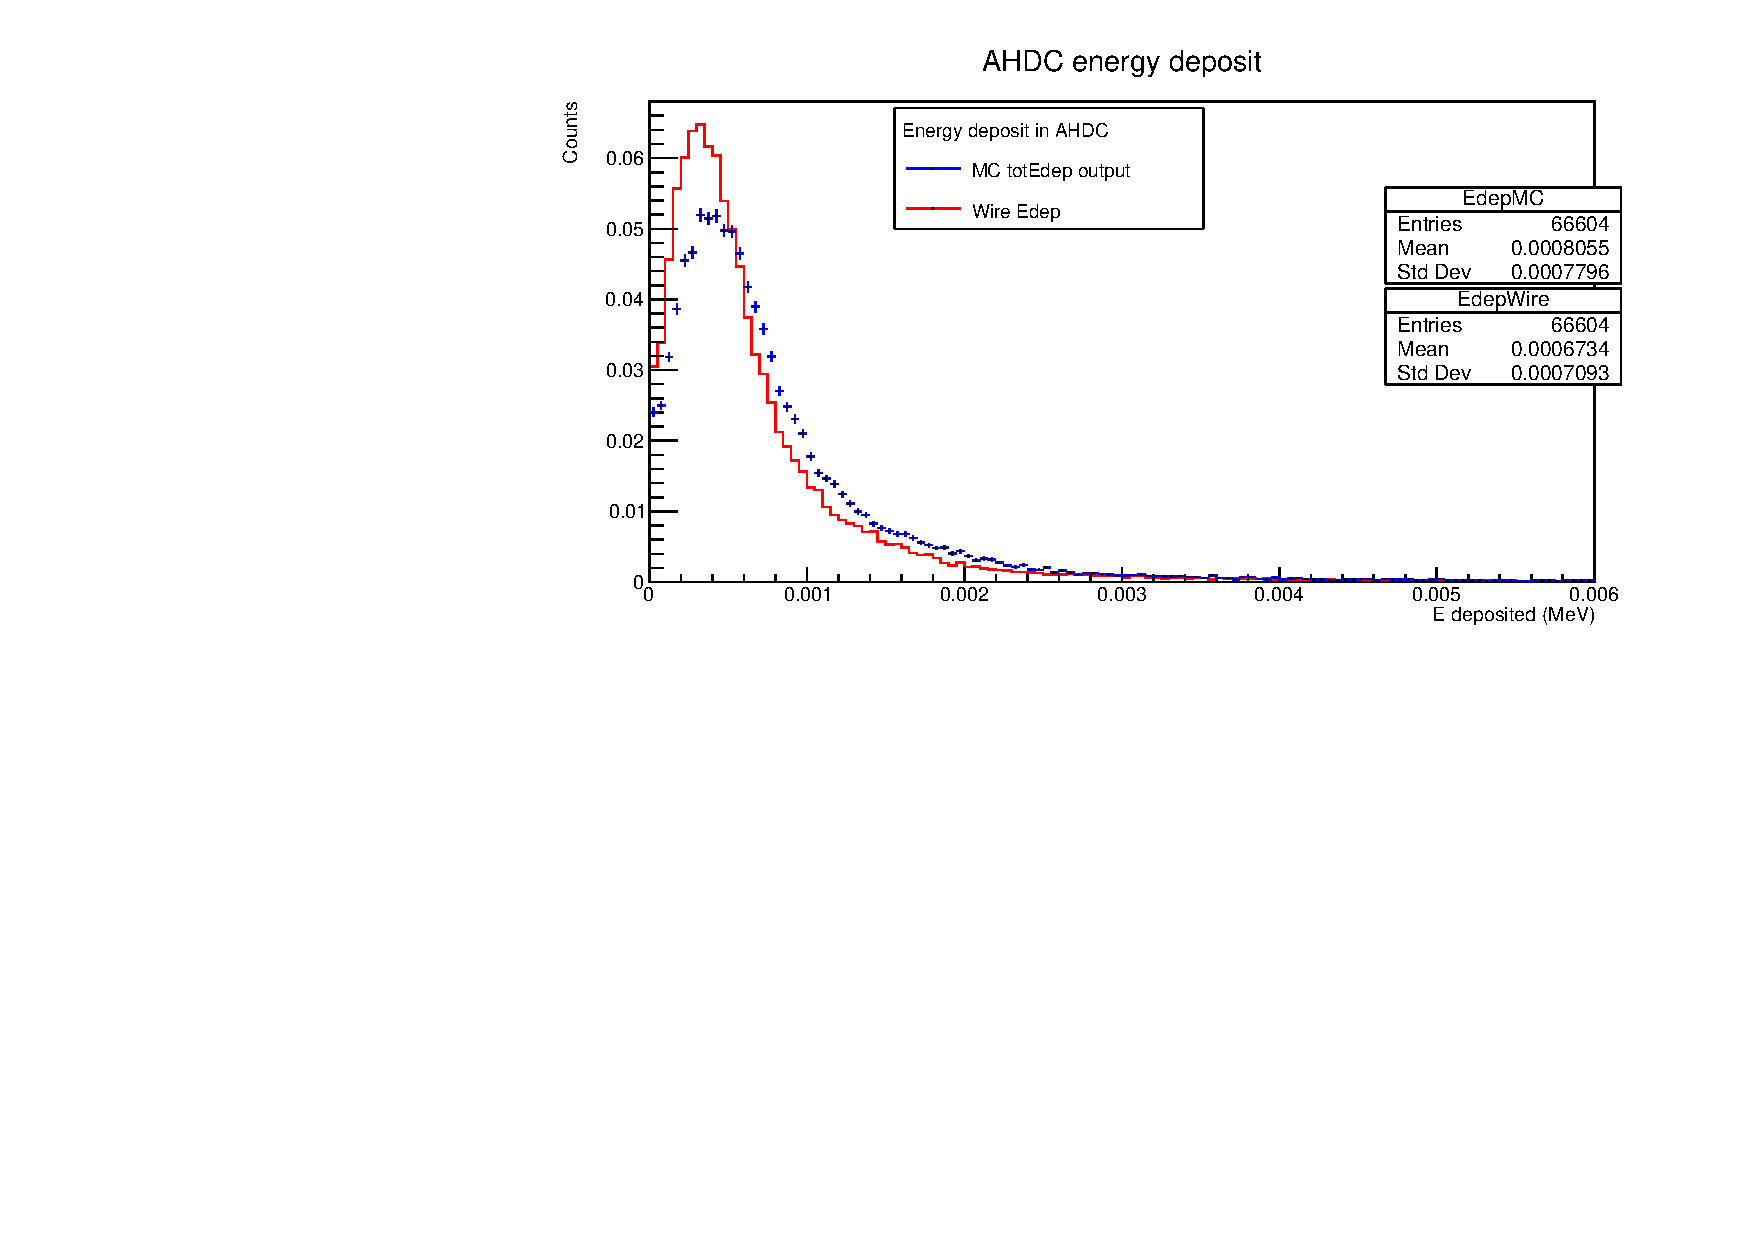
\includegraphics[width=1.0\textwidth]{AHDC_Edep_dgtzOptions.pdf}
	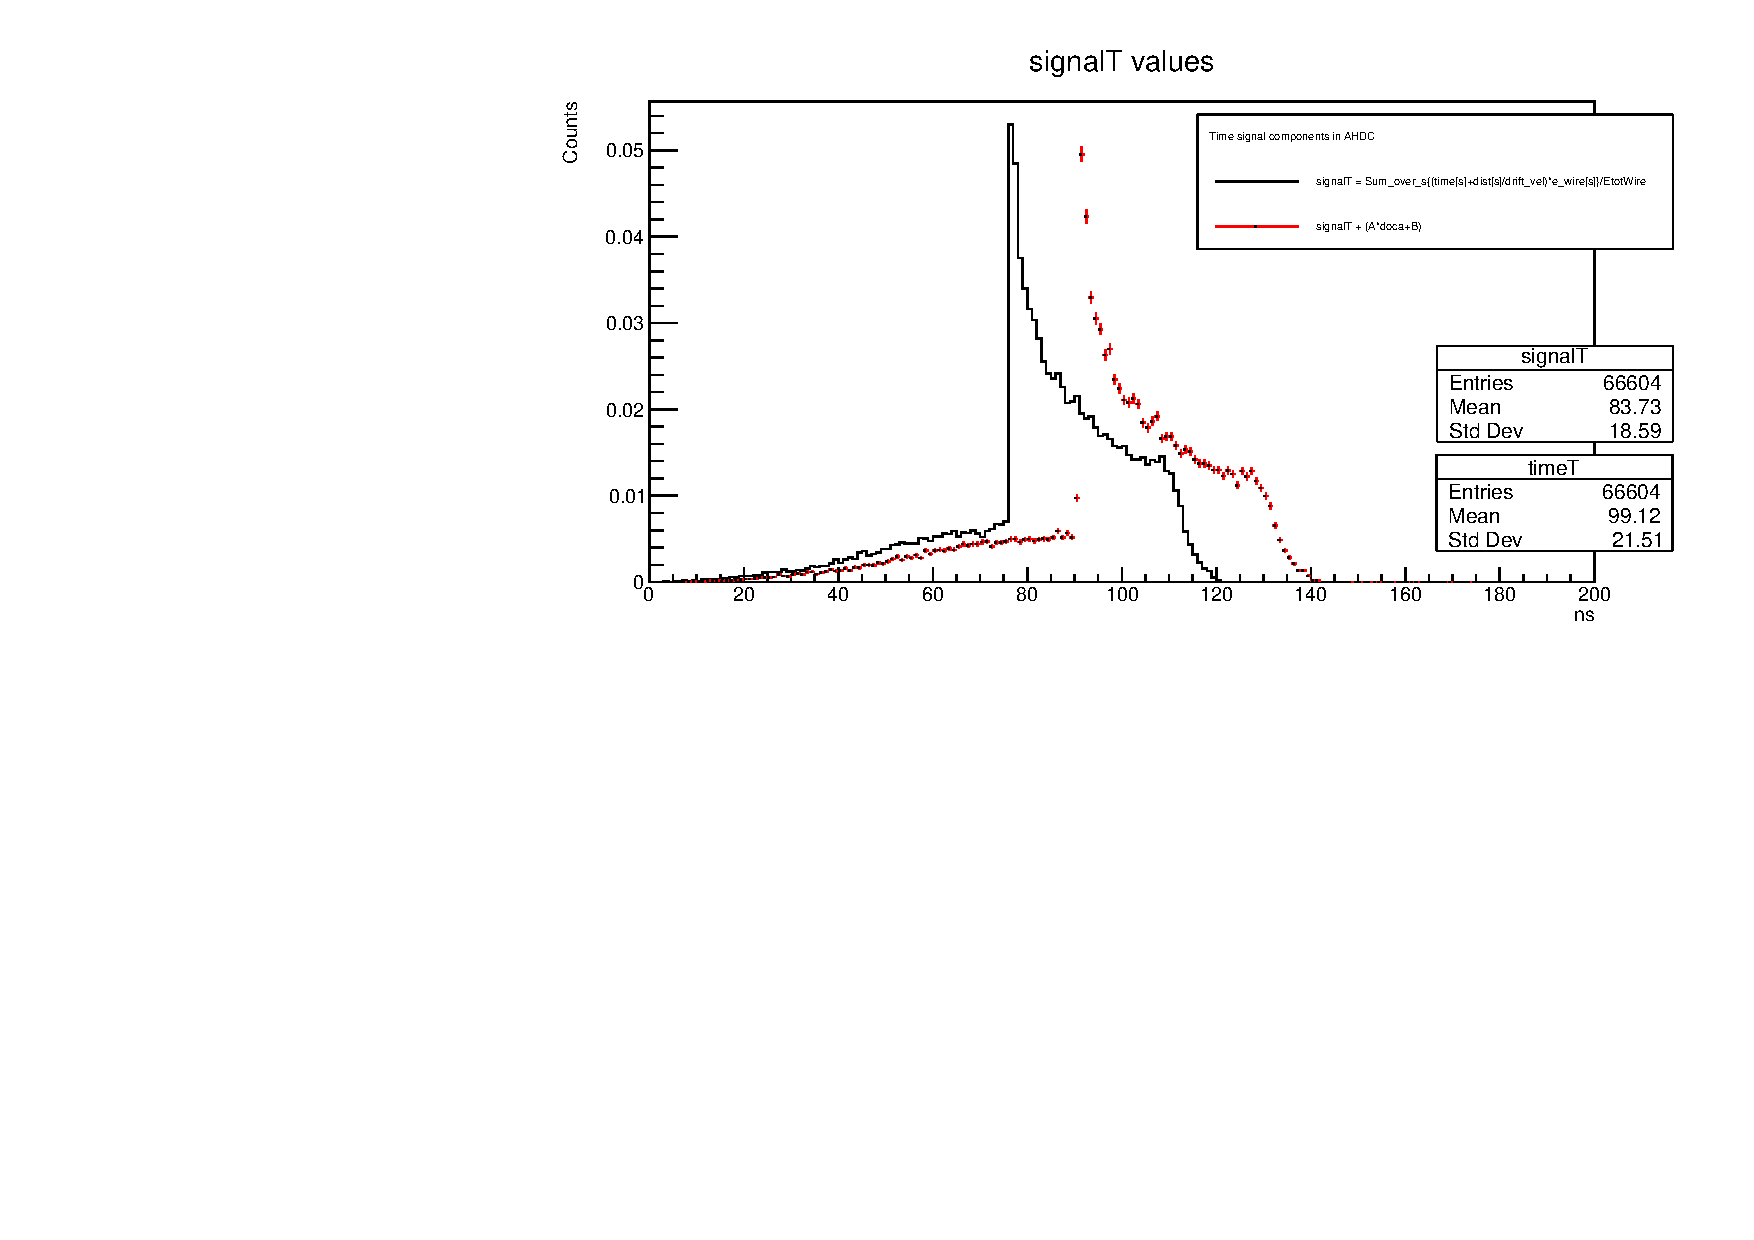
\includegraphics[width=1.0\textwidth]{signalT_ahdc.pdf}
	\caption{Wire energy output (top). Signal time output (bottom). AHDC hitprocess routine.}
	\label{fig:ahdc_dgtz}
\end{figure}	


\newpage
\section{ATOF}
The generation of ATOF digitized variables by \texttt{myatof\_hitprocess.cc} is explained here. As for AHDC, the order and the names of digitized variables inside \texttt{myatof\_hitprocess.cc} has to be exactly the same that the order and names given in  \texttt{bank.pl} when generating the geometry.

There are 18 variables included as \texttt{dgtz} output.
\begin{itemize}
	\item variable to locate where the hit happened - \texttt{sector, superlayer, layer, paddle}
	\item energies - \texttt{adc\_front, adc\_back, adc\_top}
	\item time - \texttt{tdc\_front, tdc\_back, tdc\_top}
	\item variables for checking/debug of the implementation - \texttt{time\_front, time\_back, time\_top} and \texttt{E\_tot\_Front, E\_tot\_Back, E\_tot\_Top, totEdep\_MC}
	\item the hit number - \texttt{hitn}
\end{itemize}

The computation of all these variables is done inside \texttt{myatof\_hitprocess.cc}. 

	\paragraph{Energies (MeV)}
	The split in 3 ADC outputs is due to the SiPM photomultipliers location on the ATOF paddles. 
	
	There are 2 SiPM per paddle for the superlayer \#0, one at each $Z$ end of a paddle. That are the ADC outputs named as \texttt{adc\_front, adc\_back} for the upstream and downstream SiPM coordinates.
	
	There is 1 SiPM per paddle for the superlayer \#1, located on paddle side that corresponds to the biggest radius from the $Z$ axis. This is the ADC output named as \texttt{adc\_top}. 
	
	For each hit, the distance between it and the 3 SiPM locations is computed. This distance is used to obtain the 3 ADC outputs. First, energy deposit is computed as follows:
	\begin{equation}
	EdepFront = \sum_{s=1}^{all steps} Edep[s] e^{-d_{front}/attenlength}
	\end{equation}
	
	The same procedure is done for back and top SiPMs.
	To obtain the ADC, the energy value is modified by calibration coefficients (CC). The CC are not know for the moment, arbitrary values are given in the implementation. The conversion from energy to ADC using $G4Poisson$ and $pmtPEYld$ is taken from CLAS12 FTOF and CND implementations. 
	
	\paragraph{Time (ns)}
	As for the ADC case, TDC output is splitted in 3. The \texttt{tdc\_front, tdc\_back} for superlayer \#0 paddles and \texttt{tdc\_top} for superlayer \#1 paddles. 
	
	For each step the MC truth time is taken and weighted by the deposited energy, then the sum over all the steps is divided by the total deposited energy. \\
	\begin{equation}
	time\_front = F (time_{weighted}^{front}) = \frac{\sum_{s=1}^{all steps} (time[s] + \frac{d_{front}[s]}{v_{eff}^{front}}) \times E_{front}[s]}{EdepFront}
	\end{equation}
	
	To obtain the TDC, the time value is affected by conversion coefficients. The conversion from time to TDC using $G4RandGauss::shoot(time\_front, sigma\_time)$ is taken from CLAS12 FTOF and CND implementations. The time resolution value is $sigma\_time$ and is $ = 0.1 \ ns$ now.
	Same procedure is done 3 times, one for each SiPM location.
	
Figure \ref{fig:atof_dgtz} shows the example of dgtz output that we obtain.
\begin{figure}[H]
	\centering
	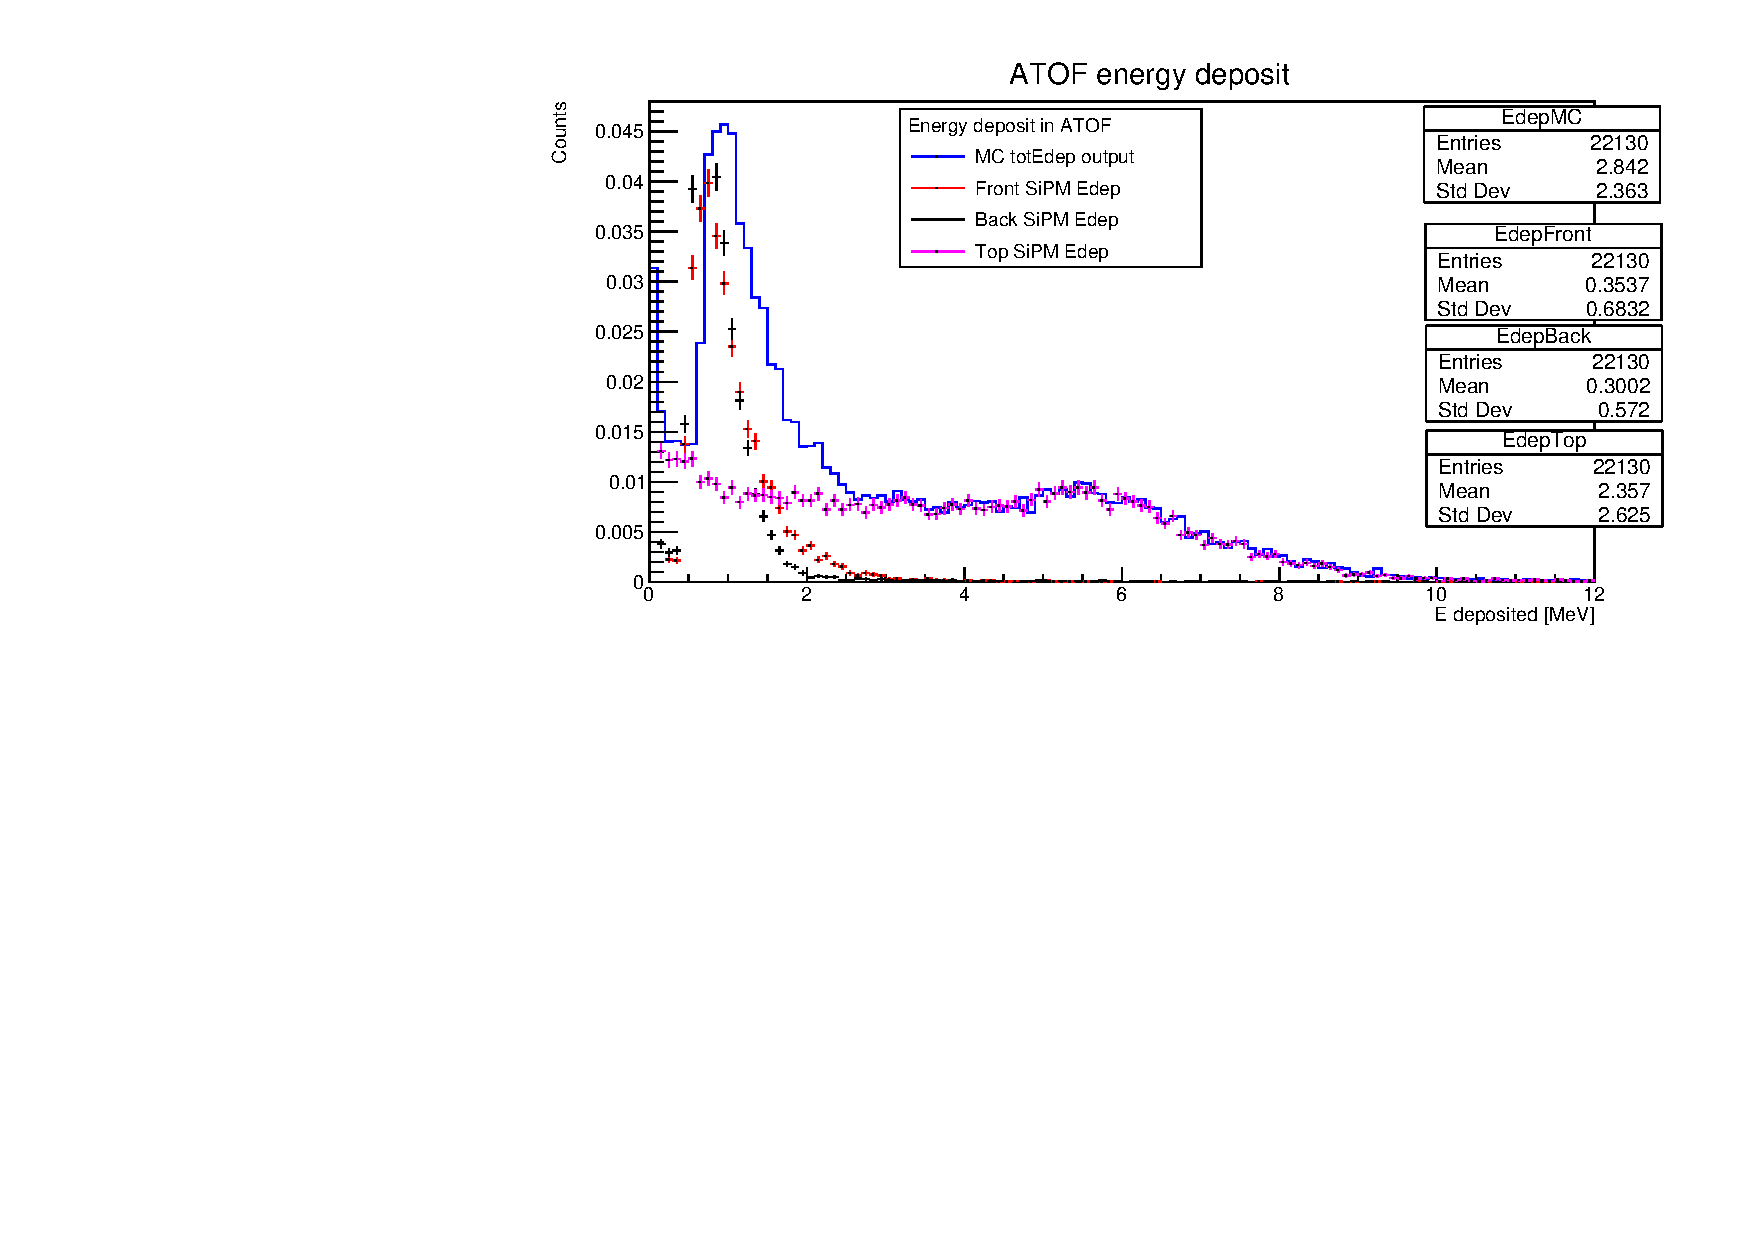
\includegraphics[width=0.8\textwidth]{ATOF_Edep_dgtzOptions.pdf}
	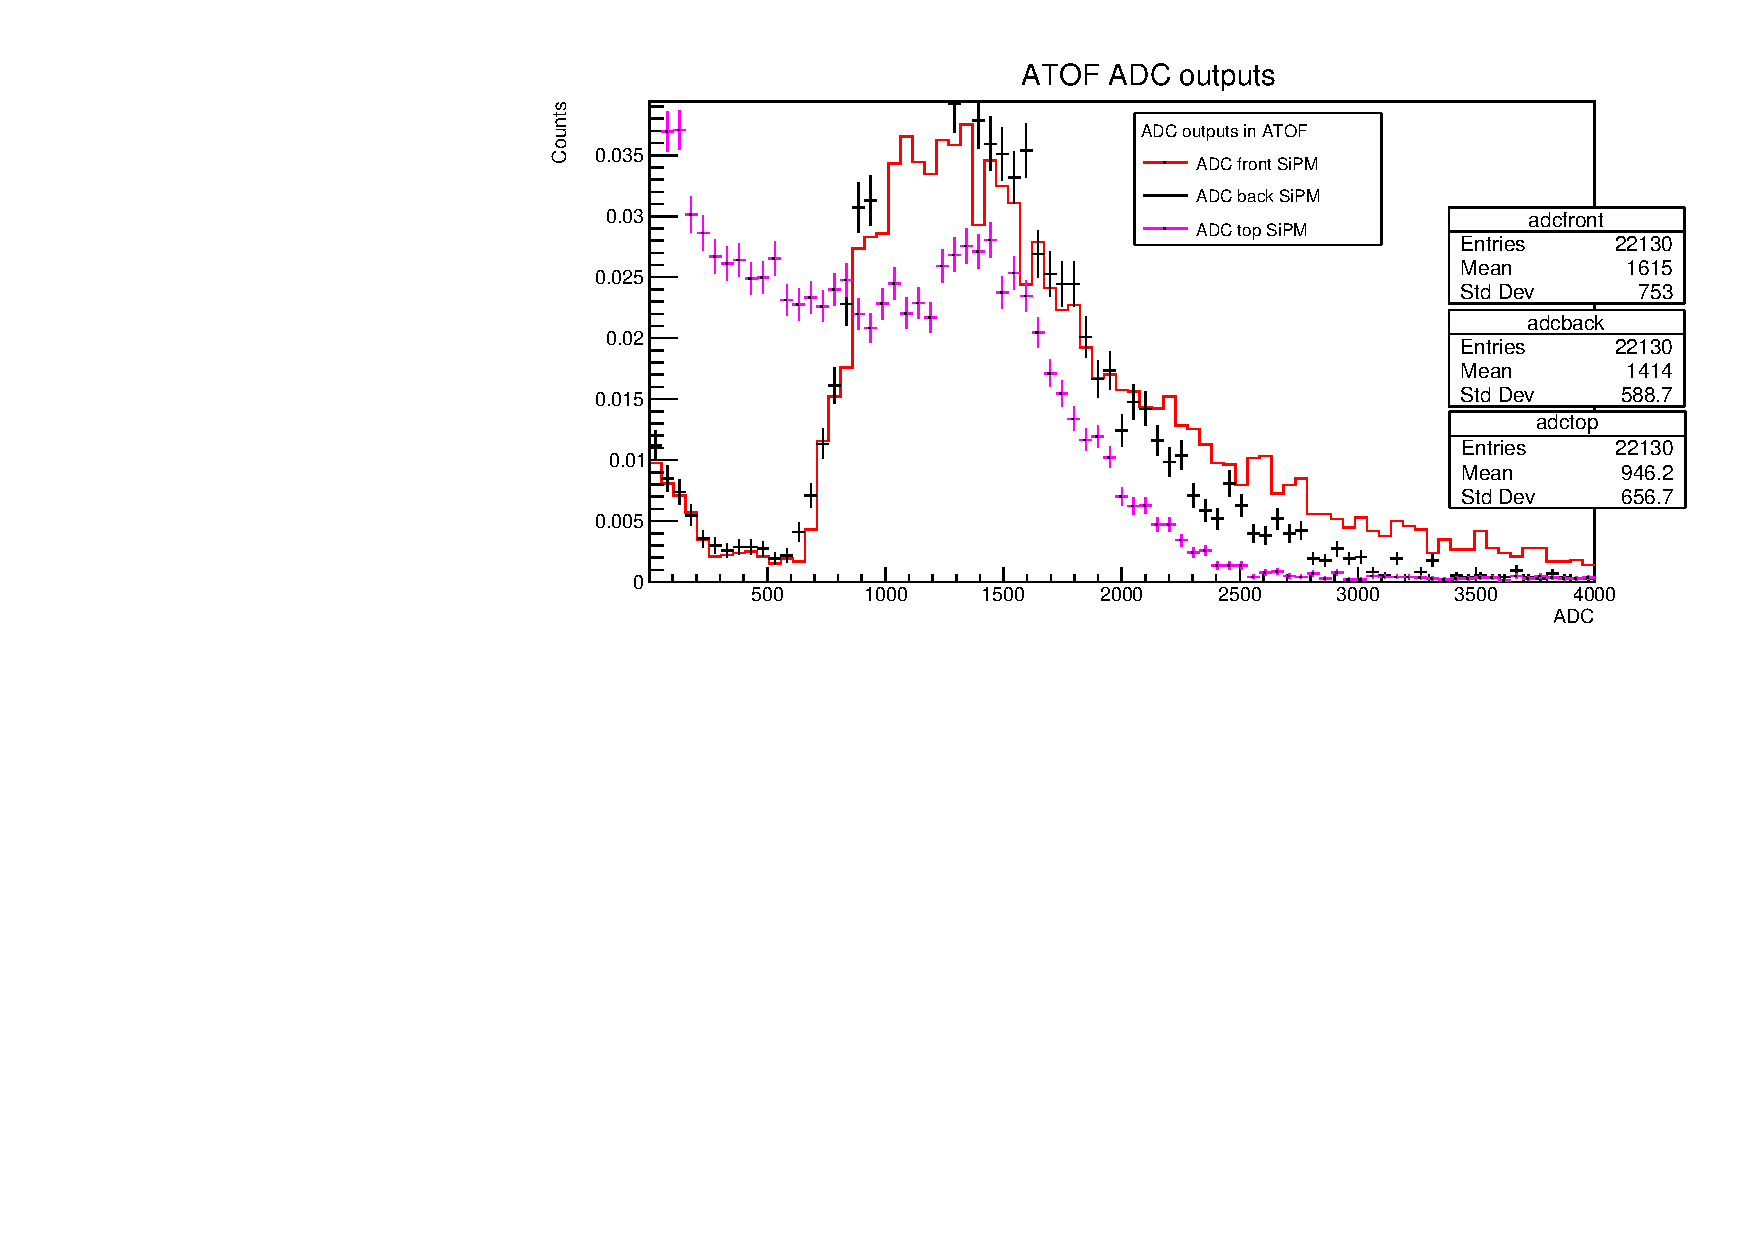
\includegraphics[width=0.8\textwidth]{ATOF_ADC_dgtzOptions.pdf}
	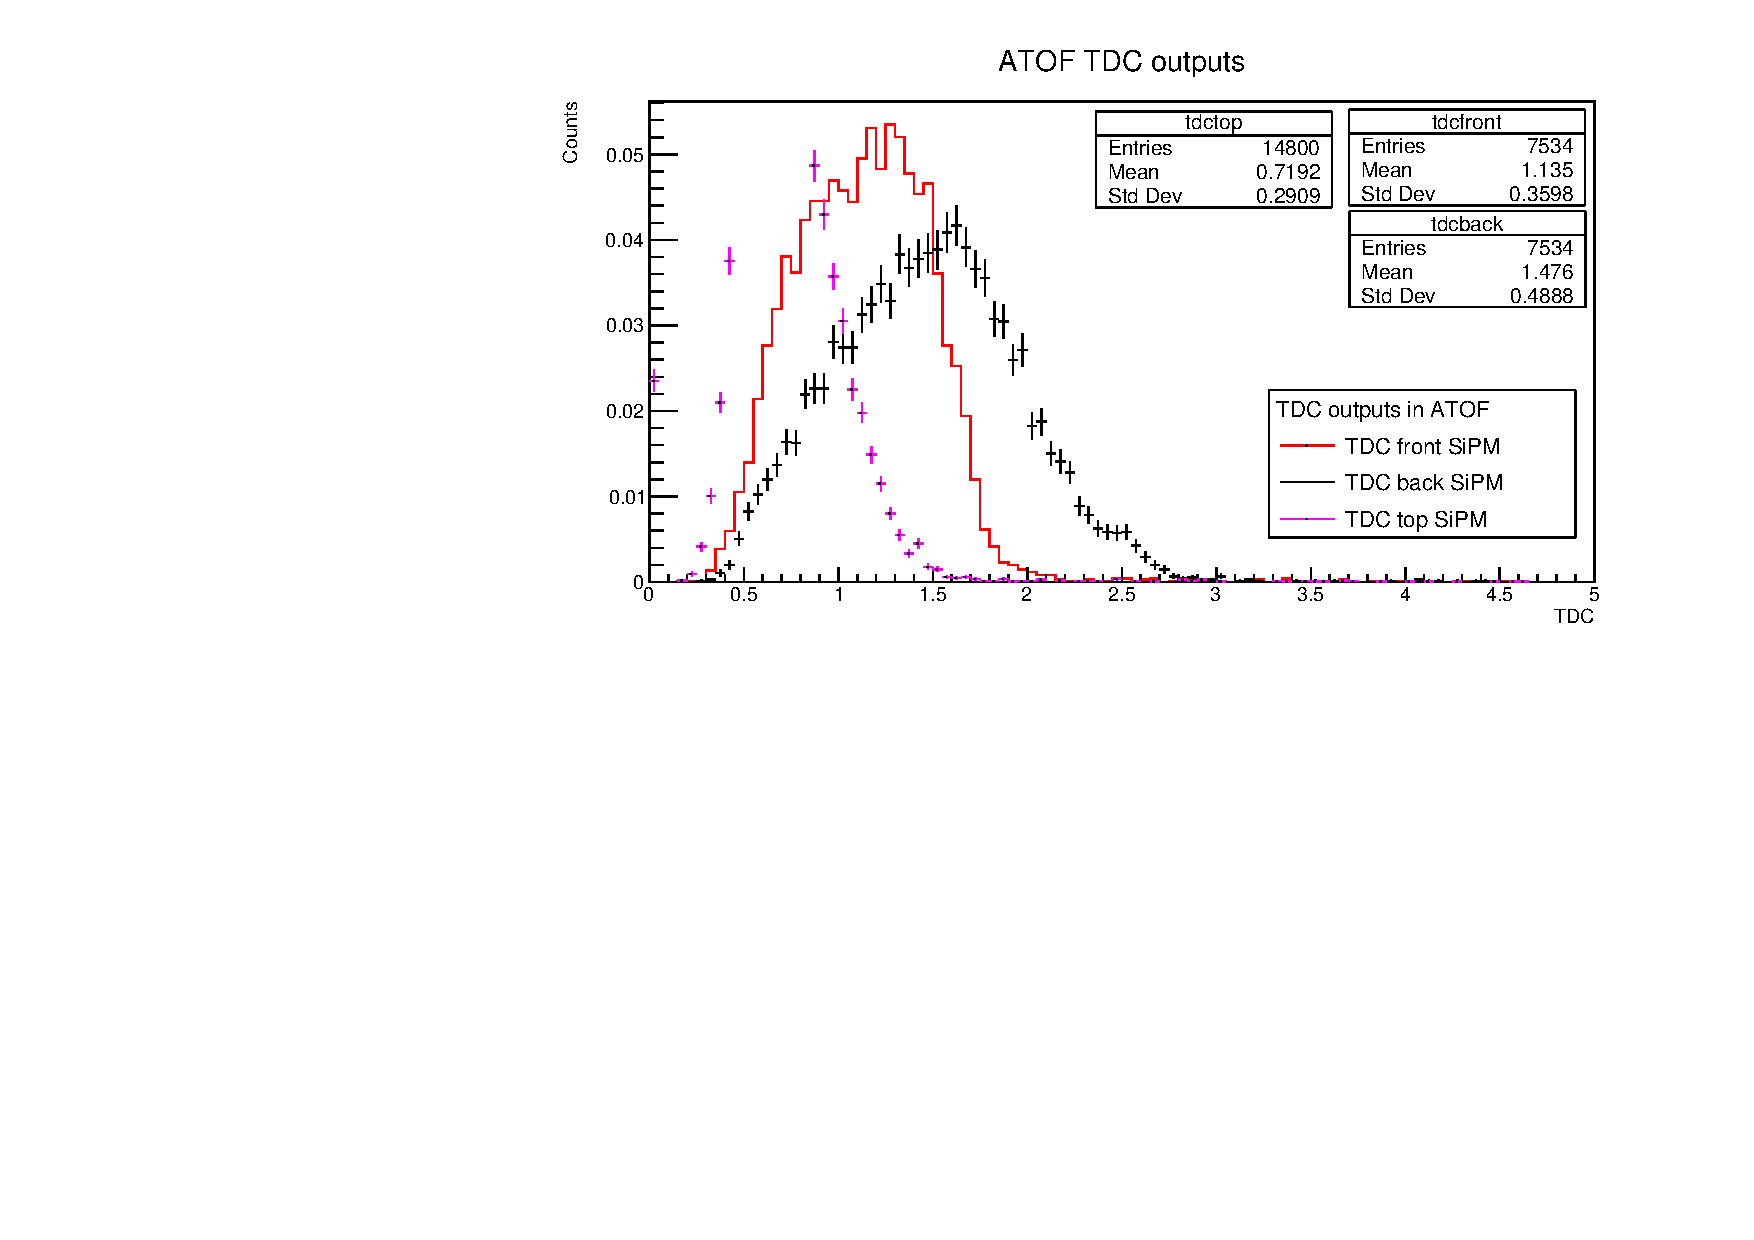
\includegraphics[width=0.8\textwidth]{ATOF_TDC_dgtzOptions.pdf}
	\caption{Deposited energy outputs: total and separation in front, back, top SiPM (top). Example of conversion to ADC values (middle). Example of TDC shape (bottom). ATOF hitprocess routine.}
	\label{fig:atof_dgtz}
\end{figure}	



\section{Conclusion}
This is the first version of digitized outputs for AHDC and ATOF. Energy and time calculation can be modified in order to be more realistic. Tests from ALTO using ALERT prototype can be used to tune the \textsl{dgtz} signals to the real life electronic outputs. Material properties such as attenuation length, electron yield, SiPM characteristics and calibration coefficients have still to be updated to the real values.

The following steps modify or add information to \textit{GEMC} source code:
\begin{enumerate}
	\item use \texttt{jeffersonlab/gemc:devel} docker container \\
		\texttt{> docker run -it --rm -v ~/myworkGemcDocker:/jlab/work/myworkGemcDocker \\ jeffersonlab/gemc:devel bash}  
	\item develope inside \texttt{/source/hitprocess/clas12/alert/ ...} and modify hitprocess calls at several other places \texttt{SConstruct} and \texttt{HitProcess\_MapRegister.cc}
	\item compilation by \texttt{>scons -j8} into  \texttt{source} directory
	\item \texttt{>./gemc} to execute the freshly compiles source
	\item if output variables or hit names are changed or new ones added, remember to update \texttt{bank.pl}, \texttt{hit.pl} with exactly the same names for \textsl{dgtz} bank and hit name!
\end{enumerate} 

